\documentclass[conference]{IEEEtran}

\usepackage{amsmath,amssymb,amsfonts} % Math
\usepackage{bm} % Bold greek letters
% \usepackage{algorithmic}
\usepackage{graphicx} % Plots
\usepackage[style=ieee]{biblatex} % Bibliography management
% \usepackage{textcomp}
\usepackage[super]{nth} % Support for nth counting, aka 1st, 2nd, ...
\usepackage{xcolor}
\usepackage{algorithm, algpseudocode} % Algorithm block
\usepackage{setspace} % Spacing in algorithm block
\usepackage{tabularx} % Good tables
\usepackage{placeins} % FloatBarrier 
\usepackage{subcaption} % Subfigures
\usepackage{svg}
\usepackage{hyperref}

\addbibresource{..\\sources.bib}

\graphicspath{{.\\figures}}

\newcommand*{\norm}[1]{\left|\left|#1\right|\right|}
\newcommand{\TODO}[1]{{\LARGE \textbf{TODO}: #1}}
\newcommand*{\x}[1][i]{x^{(#1)}_t}
\newcommand*{\xdot}[1][i]{\dot{x}^{(#1)}_{t}}
\newcommand*{\xdotdot}[1][i]{\ddot{x}^{(#1)}_t}

\newcommand*{\state}[1][i]{\mathbf{x}^{(#1)}_t}
\newcommand*{\R}[1]{\mathbf{R}^{#1}}
\newcommand*{\A}{\mathbf{A}}
\newcommand*{\C}{\mathbf{C}}
\newcommand*{\W}[1][t]{\mathbf{W_{#1}}}
\newcommand*{\V}[1][t]{\mathbf{V_{#1}}}
\newcommand*{\Q}[1][t]{\mathbf{Q_{#1}}}
\newcommand*{\thet}[1][i]{\theta^{(i)}_t}

\newcommand*{\totstate}[1][t]{\mathbf{x}_{#1}}
\newcommand*{\totu}[1][t]{\mathbf{u}_{#1}}
\newcommand*{\totmeas}[1][t]{\mathbf{y}_{#1}}
\newcommand*{\f}{\mathbf{f}}
\newcommand*{\g}{\mathbf{g}}


\begin{document}

\title{Range-Based Localization and Tracking Using Hybrid Optimization}

\author{\IEEEauthorblockN{Erik Helmer}
\IEEEauthorblockA{\textit{Department of Electrical Engineering} \\
\textit{Stanford University}\\
Palo Alto, USA \\
erik.helmer@stanford.edu}
}

\maketitle

\begin{abstract}
This project intends to investigate methods for solving the classic problem of range-based localization. It uses novel robust algorithms to find an optimal starting point, then uses faster methods for non-convex optimization in later time steps given the good initial guess. The goal is to estimate the trajectories of a group of robots over time. 

\end{abstract}

\begin{IEEEkeywords}
wireless sensor networks, localization, optimization, estimation
\end{IEEEkeywords}

\section{Introduction}
\label{sec:intro}
In a variety of applications, it is necessary to localize a group of sensors or robots. In open-air environments, this can be done with GPS. In enclosed where GPS signal is not available, it is possible to do this using a variety of SLAM techniques such as bundle adjustment or pose graph optimization (PGO). These can and have been extended to optimize over a group of robots, simultaneously determining their positions~\cite{SLAM_distributed}. However, these are dependent on a complex signal processing pipeline to extract landmark or odometry measurements to optimize over. This project intends to investigate a different approach. 

The subject of this project is an implementation and extension of a novel optimization technique for distance-based relative localization. This problem is described in figure~\ref{fig:problem_desc}.
\begin{figure}[ht]
    \centering
    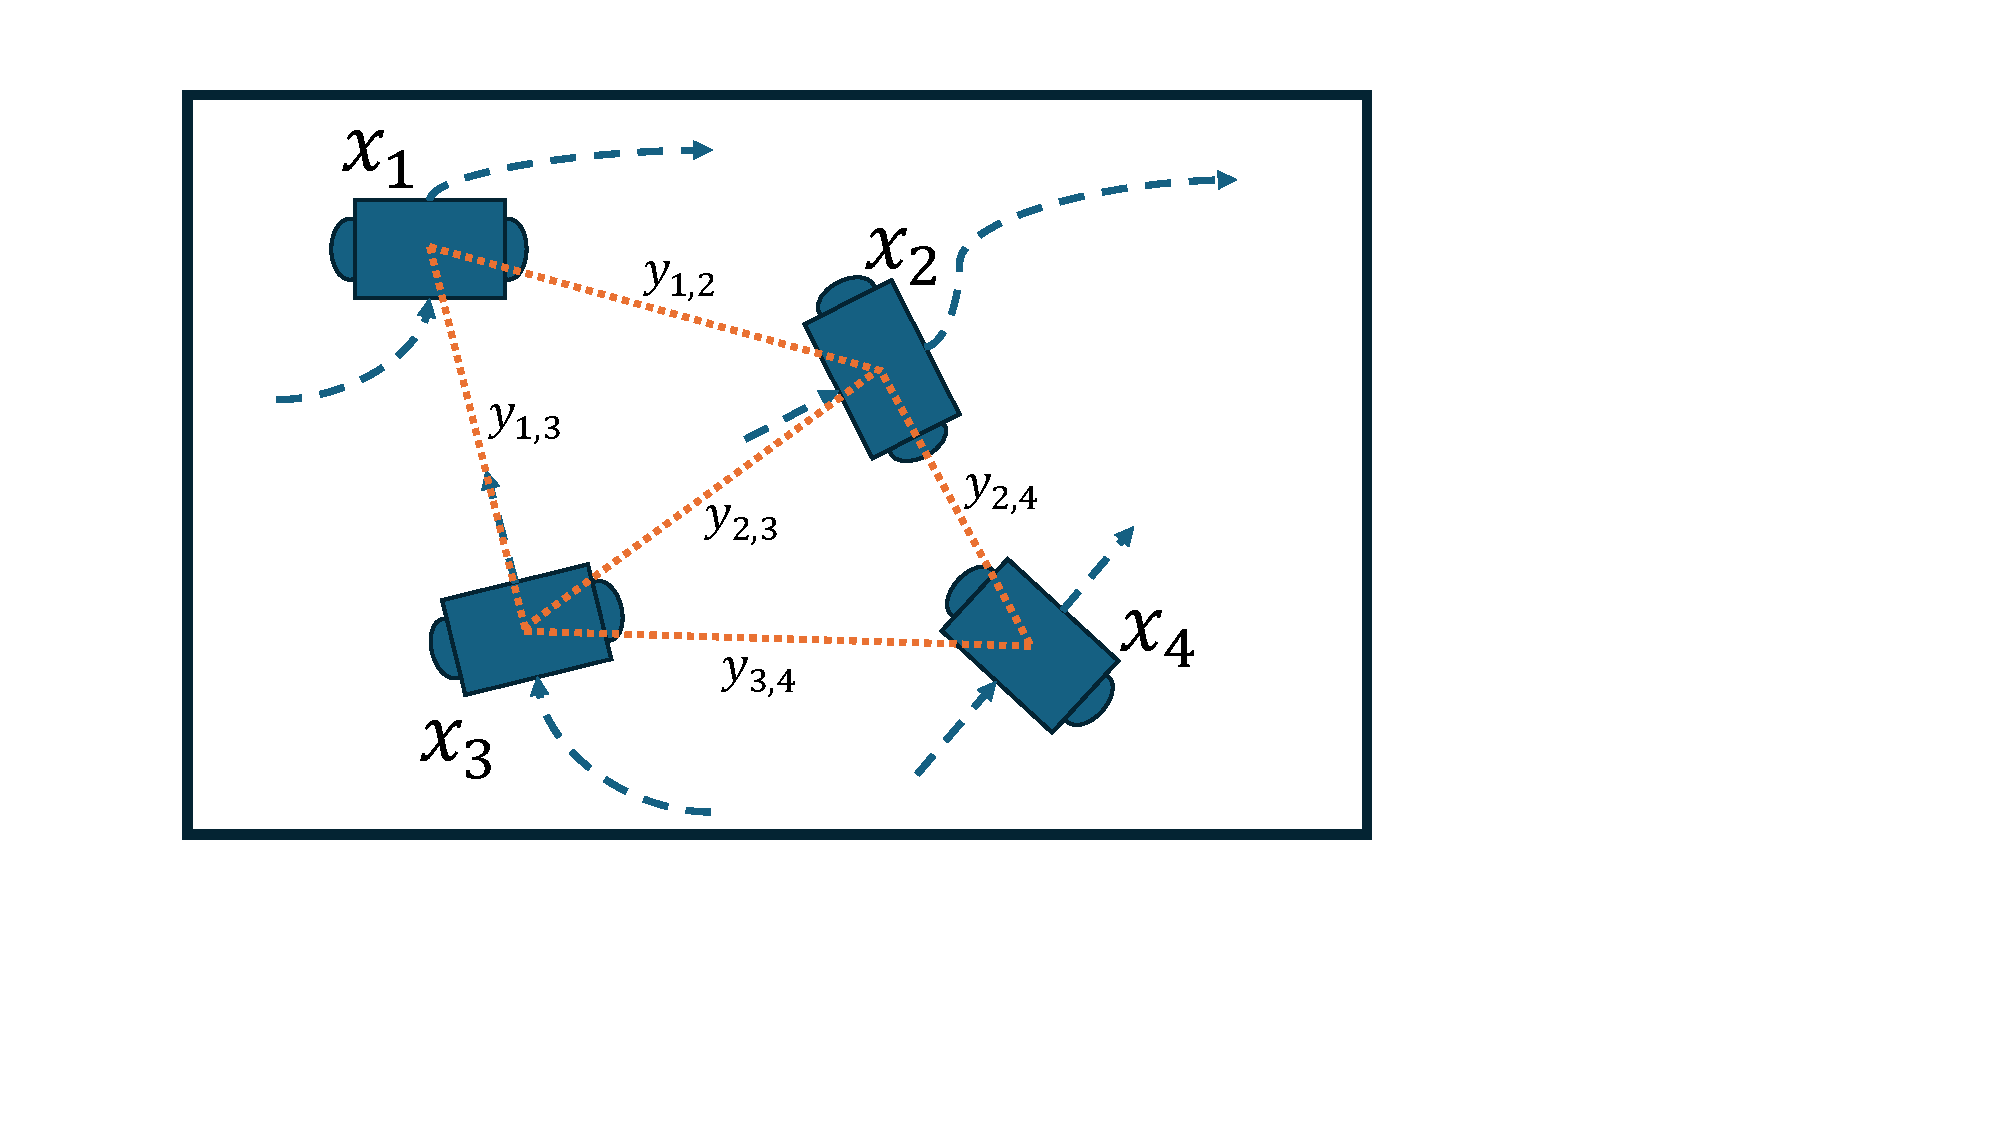
\includegraphics[width=\linewidth,trim=31mm 48mm 106mm 15mm, clip]{problem.pdf}
    \caption{Basic problem setup. In the figure, we have $N=4$ robots where $\mathbf{x}^{(i)}_t \in \mathbf{R}^n$ are the poses of the robots and $y^{(i,j)}_t \in \mathbf{R}$ are the distance measurements between them.}
    \label{fig:problem_desc}
\end{figure}

SLAM  methods usually rely on measurements of external fixed points in the scene to extract measurements. This method would instead rely on the robots measuring only distance to each other. 

Some assumptions are made of the problem. It is assumed that while the distance measurements may be noisy, they are measurements of another robot in the group and not a false measurement of the environment. We will further assume additive Gaussian noise on the measurements. This project will not investigate the distributed case, and will instead assume centralized knowledge of all robot measurements. While none of the algorithms used in this project require it to be so, we have nonetheless chosen to only investigate the two-dimensional case of the problem for simplicity. 

\section{Related Work}
\label{sec:related-work}
The problem formulated in section~\ref{sec:intro} is usually in the literature reformulated as a graph problem, see figure~\ref{fig:problem-graph}. The measurements are interpreted as the edge weights and the positions are interpreted as vertex positions. 
% \begin{figure}[ht]
%     \centering
%     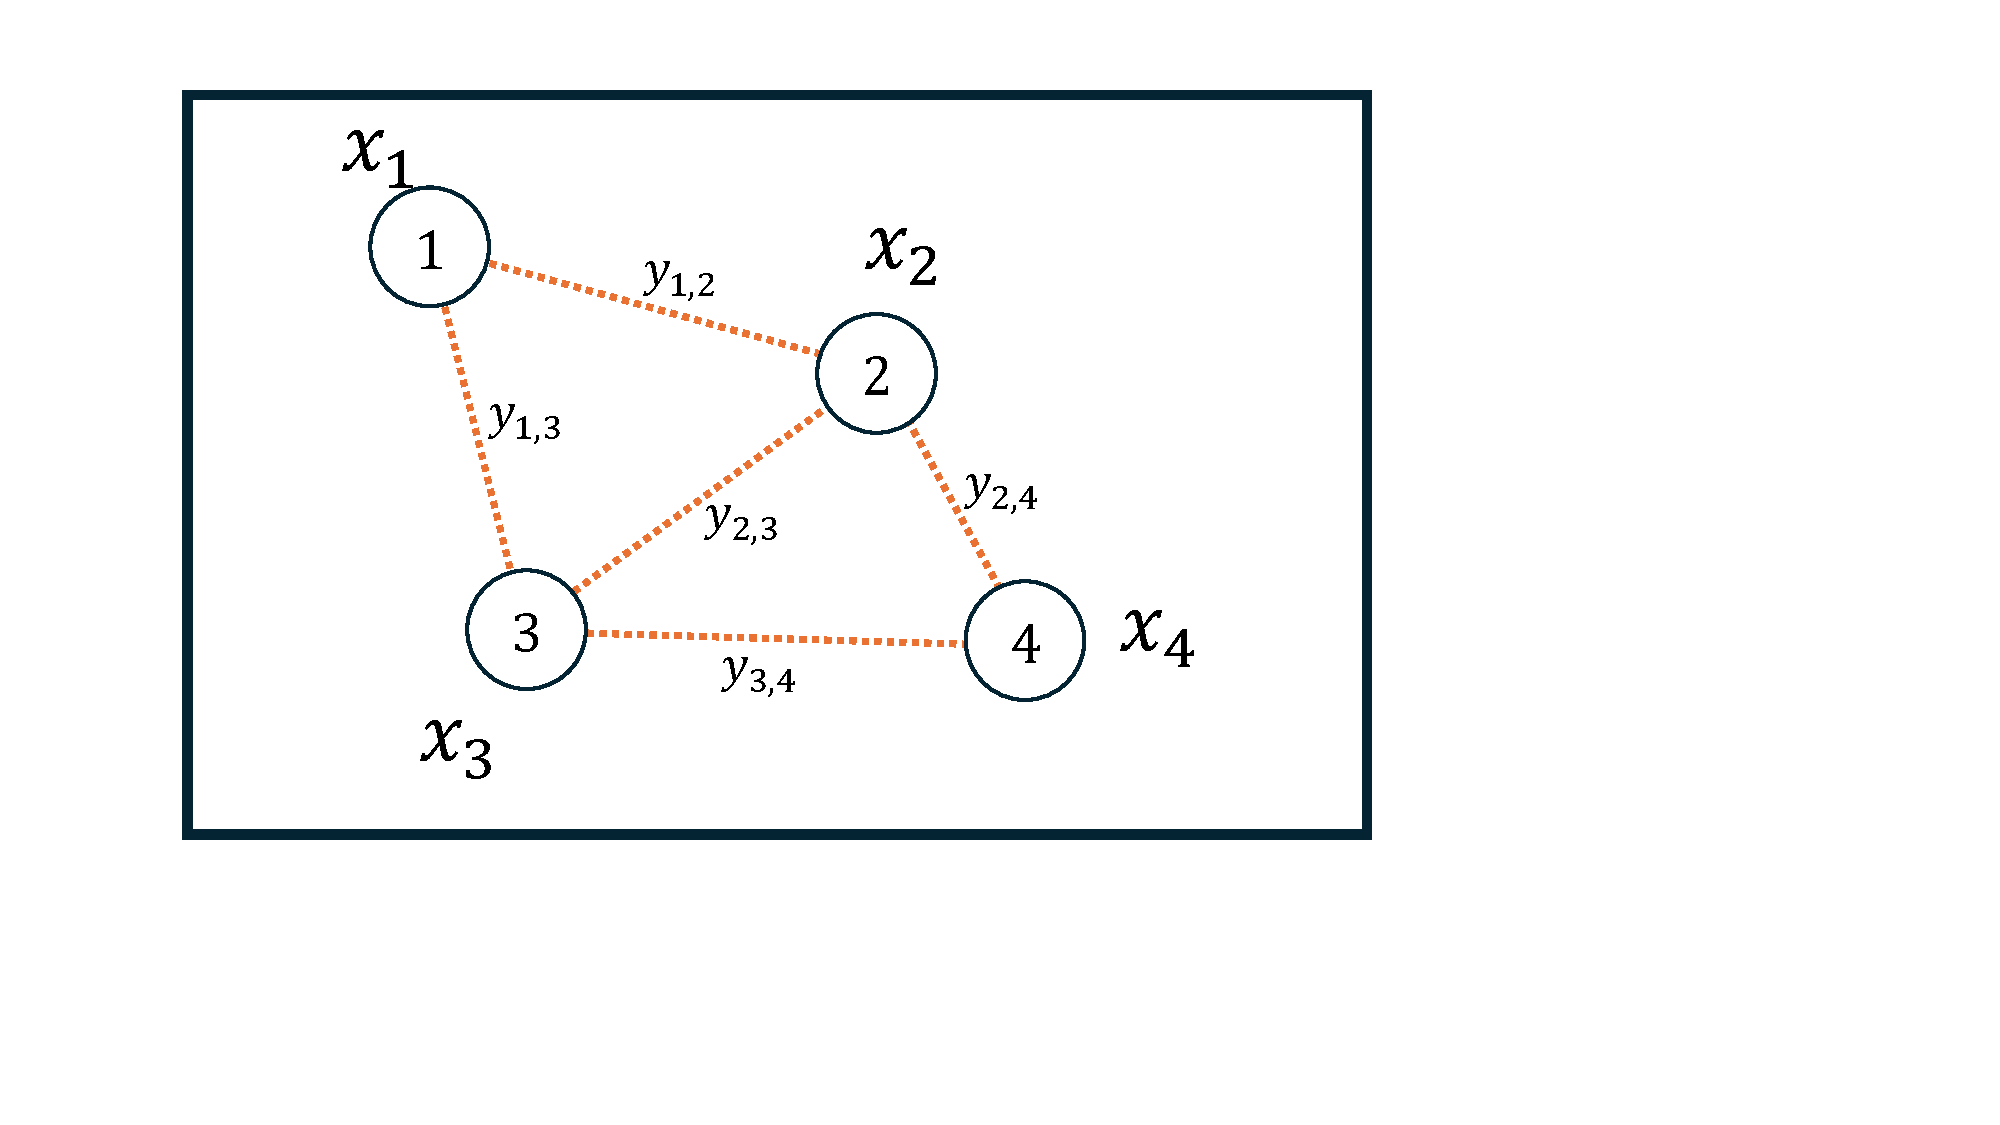
\includegraphics[width=\linewidth,trim=31mm 48mm 106mm 15mm, clip]{graph.pdf}
%     \caption{Problem reformulation. In the figure, we have a graph $\mathcal{G}=(\mathcal{V}, \mathcal{E})$ where the edges $(i, j) \in \mathcal{E}$ have weights $y_{i,j}$ and the vertices $k \in \mathcal{V}$ have positions $\bar{x}_k$.}
%     \label{fig:problem-graph}
% \end{figure}

In practice, it is rarely the case that the correspondences between robots are known without sophisticated identification algorithms using computer vision or other computationally complex methods. This is known as the anonymous localization problem, and it has been investigated by Franchi, Oriolo and Stegagno~\cite{anonymous_loc_1,anonymous_loc_2,anonymous_loc_3}. They developed a few algorithms to account for the missing correspondences by using statistical methods to simultaneously estimate multiple possible relative poses to determine the most likely correspondences. However, this markedly increases the complexity of the problem and will not be the focus of this project.

It will henceforth generally be assumed that while the measurements $y_{i,j}$ are not complete, i.e. all robots do not have measurements of every other robot, the correspondences are known. That is to say, for all measurements $y$, it is known which distance between two robots this is a measurement of. 

This problem is not new. One early approach to solve it was presented by Kruskal in \cite{Kruskal1964}. He proposed a measurement of good fit, or loss, named the stress function: 
\begin{align}
    \label{eq:kruskal-stress}
    S(\mathbf{x}^{(1)}, ..., \mathbf{x}^{(N)}) = \sum_{i,j} \left(
        \norm{\mathbf{x}^{(i)} - \mathbf{x}^{(j)}}_2 - y^{(i, j)}
    \right)^2
\end{align}
More accurately, Kruskal proposed a normalized version of equation~\ref{eq:kruskal-stress}, but for the purposes of this project the unnormalized version is sufficient. This function is non-convex, so iterative optimization algorithms such as gradient descent or ADMM generally converge to local minima, which necessitates a good initial guess. This algorithm will hereafter be called stress minimization in this paper.

In a companion paper, Kruskal provided a description of how to solve this problem using gradient descent~\cite{kruskal1964implementation}. Of interest to this project is the gradient that Kruskal determined. It should be noted that the stress function is non-differentiable and non-convex, so while Kruskal calls it a gradient, it is not necessarily so. Nonetheless, the stress minimization algorithm presented by Kruskal show empirically good results, so this this paper will continue with the slight abuse of notation. The gradient which will be used in the gradient descent variant algorithms implemented for this paper is derived from the one Kruskal presented in~\cite{kruskal1964implementation}. Given 
\begin{table}[ht]
    \centering
    \begin{tabularx}{\linewidth}{lX}
        $\mathbf{X} \in \R{2}$ & Current positions of robots \\
        $\hat{\mathbf{d}} \in \R{m}$ & Pairwise distance measurements between robots \\
        $\mathbf{d} \in \R{m}$ & Current distances between robots 
    \end{tabularx}
\end{table}
\FloatBarrier 
\noindent we get the gradient through
\begin{align}
    S^* &= \sum \left({d}_{i} - \hat{{d}}_{i}\right)^2 \\
    T^* &= \sum {d}_{i}^2 \\
    S   &= \sqrt{\frac{S^*}{T^*}} \\
    \mathbf{g}_k &= S \sum_{i} \frac{{d}_i - \hat{{d}_i}}{{d}_i} (\mathbf{X}_k - \mathbf{X}_{R(i)})
\end{align}
where $\mathbf{X}_k$ is row $k$ of $\mathbf{X}$, $\mathbf{g}_k$ is row $k$ of the gradient $\mathbf{g}$. Further, the sum is over all $i$ for which the measurement at row $i$ of $\hat{\mathbf{d}}$ is a measurement between robot $k$ and another robot $R(i)$.

In addition to how do calculate the gradient of the stress function, the paper also presents a way to determine the step sizes $\alpha_k$ in gradient descent:
\begin{align}
    \alpha_0 &\approx 0.2 \\
    S_k &= S(\mathbf{X}_k) = S(\mathbf{x}^{(1)}_k, ..., \mathbf{x}^{(N)}_k) \\
    \alpha_{k} &= \alpha_{k-1} \cdot \beta_k \cdot \gamma_k \cdot \delta_k \\
    \beta_k &= 4^{(\cos^3 \theta_k)} \\
    % \phi_k &= \frac{\left|\left|g_k\right|\right|_2\left|\left|g_{k-1}\right|\right|_2}{g_k^\top g_{k-1}} \\
    \theta_k &= (\text{Angle between last and current gradient}) \\
    \gamma_k &= \frac{1.3}{1 + (\min\{1, \frac{S_k}{S_{k-5}}\})^5} \\
    \delta_k &= \min\{1, \frac{S_k}{S_{k-1}}\}
\end{align}
This algorithm will from this point on be referred to as Kruskal's method or gradient descent with Kruskal step size. 

An alternative algorithm was proposed in~\cite{MDS_proposal} by De Leeuw. THe algorithm is called Scaling by MAjorizing a COmplicated Function (SMACOF), and it iteratively minimizes an upper bound of the stress function. Further investigated by De Leeuw in~\cite{SMACOF_convergence}, it has been proven to converge to a local minima of the stress function. However, this also requires a good initial guess to converge to a good optimum. 

These methods, while prone to local minima, can still be useful due to their simplicity when given a sufficiently good initial guess. 

In the field of sensor network localization, meaning many agents are deployed in an environment without knowledge of their positions, this problem has also been investigated. The main distinction with the robot localization problem is that authors generally assume that at least some positions known as anchors are known~\cite{WSN_collaborative,WSN_localization_techniques,optimization_WSN,WSN_stochastic}. 

% Authors in these fields present additional methods of solving this problem, with different advantages and drawbacks. One technique is Particle Swarm Optimization (PSO), where a collection of particles explore the n-dimensional space to find optima~\cite{WSN_particles}. Building on this, Zhou and Chen gave a stochastic approach in~\cite{WSN_stochastic}, which finds the global optimum with high probability. 

Recently, there has been some advancements in solving the distance-based localization problem. An algorithm developed by Halsted and Schwager dubbed the Riemannian Elevator has been proposed which has better guarantees than either stress minimization or SMACOF. This method relies on a tight modification of the stress minimization problem. The weighted stress minimization problem, where the distances have weights inversely proportional to their noise variance, given by 
\begin{align}
    \min_{\mathbf{X} \in \R{n \times d}} \sum_{i, j} \frac{w_{ij}}{2}\left(\norm{\mathbf{x}_i - \mathbf{x}_j} - \hat{d}_{ij}\right)^2
\end{align}
is modified by adding the unit vectors $y_{ij}$ and jointly optimizing
\begin{align}
    \min_{\substack{
        \mathbf{X} \in \R{n \times d} \\
        \mathbf{Y} \in (\mathcal{S}^{d-1})^m
    }} 
    \sum_{i, j} \frac{w_{ij}}{2}\norm{\mathbf{x}_i - \mathbf{x}_j - \hat{d}_{ij}\mathbf{y}_{ij}}^2
    \label{eq:re-prob3}
\end{align}
where $(\mathcal{S}^{d-1})^m$ the set of $m \times d$ matrices with unit vector rows, or equivalently, an oblique manifold. The following equivalent form of equation~\ref{eq:re-prob3} is the basis for the Riemannian elevator algorithm:
\begin{align}
    \min_{\mathbf{Y} \in (\mathcal{S}^{d-1})^m}
    \text{tr}(\mathbf{Q Y Y}^\top)
    \label{eq:re-prob4}
\end{align}
where 
\begin{align}
    \mathbf{Q} &= \hat{\mathbf{D}}^2 \mathbf{(W - WC(C^\top W C)^\dagger C^\top W)}
\end{align}
where $\mathbf{C}$ is the graph incidence matrix and where $\mathbf{W}$ and $\hat{\mathbf{D}}$ have $w_{ij}$ and $\hat{{d}}_{ij}$ respectively on their diagonals. This problem is relaxed by increasing the dimension of $\mathbf{Y}$ to $(\mathcal{S}^{m-1})^m$, then it is reparametrized into an SDP. By solving this SDP problem and then projecting the solution to $\mathbf{Y} \in (\mathcal{S}^{d-1})^m$, we get a good initial guess to the problem in equation~\ref{eq:re-prob4}, which can then be solved to a local minima with manifold optimization libraries~\cite{pymanopt}.

\section{Problem Statement}
\label{sec:prob-statement}
This project will combine some earlier approaches described in section~\ref{sec:related-work} to investigate whether this can improve estimation performance. The problem to be investigated, as well as the notation to be used, is described below.

\subsection{State-Space Model}
As described in section~\ref{sec:intro}, this projects seeks to investigate the problem of $n$ robots moving around in an unknown open space. The dynamics of the robots will be assumed to be \nth{1} order differential drive robot, which are robots controlled by speed $v$ and angular velocity $\omega$. This means that for each robot $i$ at time step $t$ we have 
\begin{align}
    \state = \begin{bmatrix}
        \x \\ \theta
    \end{bmatrix}
    \in \R{3} \quad \text{with} \quad \x \in \R{2}, \thet \in \R{}
\end{align}
which gives the total state
\begin{align}
    \state = \begin{bmatrix}
        \state[1] \\ \vdots \\ \state[n] 
    \end{bmatrix}
    \in \R{3n}
\end{align}

To estimate the state $\totstate$ over time we will use a extended Kalman filter (EKF). However, it will not use the distances between the robots as measurement variable. Instead, it will use the estimated positions that the optimizer algorithms determine. All robots operate independently, but we will use a single filter to estimate all of their states. With this said, update equations for a single robot $i$ are defined, below where the index $(i)$ is dropped for readability:
\begin{align}
    \totstate[t+1] &= \f(\totstate, \totu) + \W \\
    \totmeas[t+1] &= \g(\totstate) + \V
\end{align}
where
\begin{align}
    % \f(\totstate, \totu) &= \begin{bmatrix}
    %     f(\state[1], \totu^{(1)}) \\ \vdots \\ f(\state[n], \totu^{(n)})
    % \end{bmatrix} \\
    f(\totstate, \totu) &= \totstate +\Delta t
    \begin{bmatrix} 
        v \cos \theta_t \\ v \sin \theta_t \\ \omega_t
    \end{bmatrix}\\
    % \g(\totstate) &= \begin{bmatrix}
    %     g(\state[1]) \\ \vdots \\ g(\state[n])
    % \end{bmatrix} \\
    g(\totstate) &= \begin{bmatrix}
        1 & 0 & 0 \\
        0 & 1 & 0
    \end{bmatrix} \totstate \\
    \W &\sim \text{GWN} (0, \Q) \\
    \V &\sim \text{GWN} (0, \R) 
\end{align}
and where $\W$ is uncorrelated with $\V$, as well as both being uncorrelated with noise in different robots. By linearizing $f$, we get the Jacobian matrices needed by the EKF:
\begin{align}
    \mathbf{F}_t &=\begin{bmatrix}
        1 & 0 & -\Delta t v_{t} \sin(\hat{\theta}_{t \mid t}) \\
        0 & 1 & \Delta t v_{t} \cos(\hat{\theta}_{t \mid t}) \\
        0 & 0 & 1
    \end{bmatrix} \\
    \mathbf{H}_t &= \begin{bmatrix}
        1 & 0 & 0 \\
        0 & 1 & 0
    \end{bmatrix}
\end{align}
where $\hat{\theta}_{t \mid t}$ is the Kalman estimate of $\theta_t$ given measurements $\totmeas$.

\subsection{Graph Optimization} \label{sec:graphs}
% $\exists (i, j) \notin \mathcal{E}$
The positions of the robots as well as the distance measurements are modeled as a directed graph $\mathcal{G} = (\mathcal{V}, \mathcal{E})$, with $n$ vertices $i \in \mathcal{V}$ and $m$ edges $(i, j) \in \mathcal{E}$. An example configuration is shown in figure~\ref{fig:problem-graph}.
\begin{figure}[ht]
    \centering
    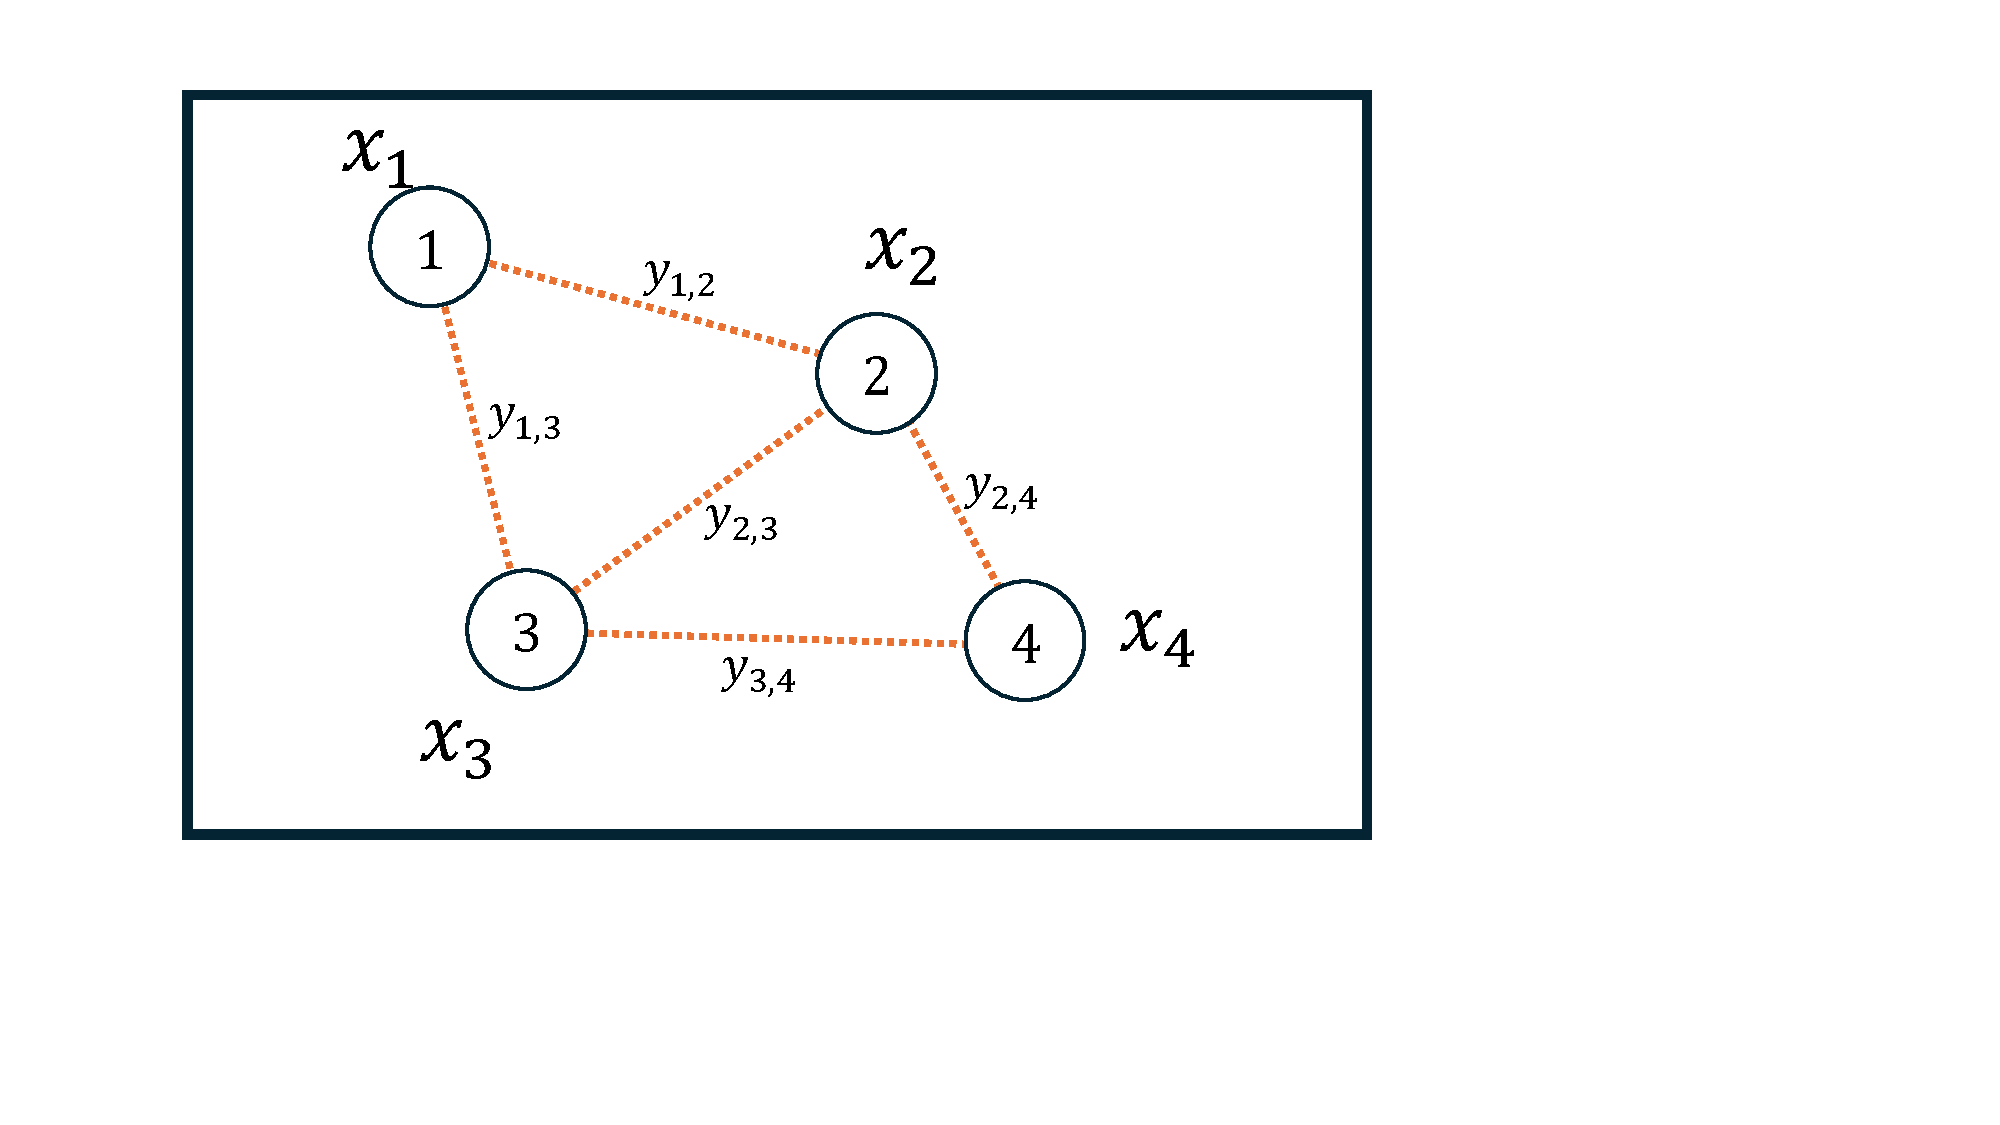
\includegraphics[width=\linewidth,trim=31mm 48mm 106mm 15mm, clip]{graph.pdf}
    \caption{Problem reformulation. In the figure, we have a graph $\mathcal{G}=(\mathcal{V}, \mathcal{E})$ where the directed edges $(i, j) \in \mathcal{E}$ have weights $l_{i,j}$ and the vertices $k \in \mathcal{V}$ have positions $x^{(k)}_t$.}
    \label{fig:problem-graph} 
\end{figure}
As described in section~\ref{sec:related-work}, this is a non-convex with no known efficient global solver. However, the Riemannian Elevator~\cite{R_elevator} provides an approximate solution as well as a non-trivial lower bound on the problem which we can use to determine the quality of the solution. Given this, we can approximately solve the localization problem for the initial positions. The estimates can be further refined using gradient descent on the stress minimization problem as described in previous sections. 

We use the notation defined in table~\ref{tab:notation} below to describe the graph and the data collected from it.
\FloatBarrier
\begin{table}[ht]
    \centering
    \caption{Additional definitions}
    \label{tab:notation}
    \begin{tabularx}{\linewidth}{lX}
        $\mathbf{J}_t \in \R{m \times 2}$ & 
        \textit{Connectivity matrix}.  Each row $(i, j)\in\mathcal{E}$ represents a directed edge of the graph. \\
        $\mathbf{y}_t \in \R{m}$ & 
        \textit{Measurement vector}. Each row $k$ is the distance measurement between the two nodes at row $k$ in $\mathbf{J}_t$. \\
        $\bm{\psi}_t \in \R{m}$ &
        \textit{Noise variance vector}. Each row $k$ is the variance of the noise measurement at row $k$ in $\mathbf{y}_t$. 
    \end{tabularx}
\end{table}

\subsection{Coordinate System}
Any solution to the stress minimization problem, either local or global is not unique. Since the stress function is invariant under translation, rotation, and mirroring, there is no way to determine a coordinate system matching some world coordinates. Therefore, any chosen coordinate system is as valid as any other. Initially, the Riemannian elevator is used to get estimates of the positions of the robots. This initial guess gives us the coordinate system to use in future time steps. However, when tracking the positions over longer a longer time horizon, it probable that the coordinate system will begin to drift. This means that, even though a point may have the same coordinates at two different time steps, $x^{(i)}_t = x^{(i)}_\tau$ for $t \neq \tau$, the real robot might not be at the same position at those two time steps. This is a fundamental limitation of the problem setup, as there is no measurements of the outside world. To remedy this, outside anchors could be provided which would both give a reference coordinate frame, as well as enable other localization algorithms like traditional SLAM. 

Ultimately, these are issues innate to the chosen problem, and even if the relative localization problem was solved globally, they would still persist. As such, we make no effort to solve these as the relative localization problem remains interesting regardless of limitations.

% \subsection{Unbiased Coordinates}
% Solving the localization problem, be it through the Riemannian Elevator or through stress minimization, is not enough. Since the stress function is invariant under translation, rotation, and mirroring, we need some canonical way of representing coordinates. For this, we use the mean and the SVD of the point list.

% Given a minimum of the stress function at a time $t$
% \begin{align}
%     \mathbf{X}_t = \begin{bmatrix}
%         (\x[1])^\top \\ \vdots \\ (\x[n])^\top
%     \end{bmatrix}
% \end{align}
% we subtract the mean from each point to get the same set of points centered at the origin.
% \begin{align}
%     \tilde{\mathbf{X}}_t = \begin{bmatrix}
%         (\x[1])^\top - \mu_{x_t}^\top \\ \vdots \\ (\x[n])^\top - \mu_{x_t}^\top
%     \end{bmatrix}
% \end{align}
% To cancel out rotation we determine the SVD and get 
% \begin{align}
%     U_t &\in \R{m \times 2} \\
%     \Sigma_t &\in \R{2 \times 2} \\
%     V_t &\in \R{2 \times 2}
% \end{align}
% Assuming that the two singular values are distinct, this is unique up to scaling by $\pm 1$ on the columns of $U_t$ and $V_t$. If we interpret $V_t$ as a basis for the 

% This means that the matrix 
% \begin{align}
%     U_t \Sigma_t V_t^\top V_t = U_t \Sigma_t
% \end{align}

\subsection{Algorithm Description}
With the content in previous sections, we can now define algorithm~\ref{algo:estimation}, the online estimation algorithm. For conciseness, we define the function $\text{RE}(C, \tilde{D}, W)$ the output of the Riemannian elevator, and $\text{KA}(\hat{\mathbf{x}}_{t \mid t-1}, \mathbf{y}_t, \bm{\psi}_t)$ as the output of gradient descent using Kruskal's algorithm. 



\begin{algorithm}
    \caption{Online estimation}\label{algo:estimation}
    \textbf{Inputs:} Connectivity matrix $\mathbf{J}_0$, measurement vector $\mathbf{y}_0$, noise power vector $\bm{\psi}_0$
    
    \textbf{Initialize:} Get an initial guess
    \begingroup\setstretch{1.2} % Increase line spacing
    \begin{algorithmic}[1]
        \Statex \underline{Find initial guess with Riemannian elevator}
        \State Construct matrices $C$, $\tilde{D}$, and $W$, see \cite{R_elevator}
        \State $\hat{\mathbf{X}}_0 \ \leftarrow\ \text{RE}(C, \tilde{D}, W)$
        \State Recover $\hat{\mathbf{x}}_{0 \mid 0} \in \R{3n}$ from $\hat{\mathbf{X}}_0 \in \R{n \times 2}$, assuming $\hat{\theta}^{(i)} = 0$ with high uncertainty.
    \end{algorithmic}

    \textbf{Track:} Continuously track the states
    \begin{algorithmic}[1]
        \Statex \underline{Predict}
        \State $\hat{\mathbf{x}}_{t \mid t-1} = \mathbf{f}(\hat{\mathbf{x}}_{t-1 \mid t-1}, \mathbf{u}_{t-1})$
        \State $\mathbf{P}_{t \mid t-1} = \mathbf{F}_t \mathbf{P}_{t-1 \mid t-1} \mathbf{F}_t^\top + \mathbf{Q}_t$
        \Statex \underline{Measure}
        \State Collect distance measurements $\mathbf{y}_t$
        \State Get position measurements $\mathbf{z}_t = \text{KA}(\hat{\mathbf{x}}_{t \mid t-1}, \mathbf{y}_t, \bm{\psi}_t)$ and corresponding matrices and vectors $\mathbf{J}_t$, $\mathbf{L}_t$, $\bm{\psi}_t$
        \Statex \underline{Update}
        \State $\mathbf{K}_t = \mathbf{P}_{t \mid t-1} \mathbf{H}^\top_t (\mathbf{H}_t \mathbf{P}_{t \mid t-1} \mathbf{H}_t^\top + \mathbf{R}_t)^{-1}$
        \State $\hat{\mathbf{x}}_{t \mid t} = \hat{\mathbf{x}}_{t\mid t-1} + \mathbf{K}_t (\mathbf{z}_t - \mathbf{g}(\hat{\mathbf{x}}_{t \mid t-1}))$
        \State $\mathbf{P}_{t \mid t} = (\mathbf{I} - \mathbf{K}_t \mathbf{H}_t) \mathbf{P}_{t \mid t-1}$
        \Statex \underline{Repeat}: Go to \underline{Predict}
    \end{algorithmic}
    \endgroup
\end{algorithm}


\section{Pipeline}
\label{sec:pipeline}
The pipeline for estimating the state over time uses two different optimization techniques as well as an extended Kalman filter. To initialize the estimation process, the Riemannian elevator algorithm is run once to generate estimations of the positions of the robots based only on distance measurements. These estimations are in practice never optimal points of the stress function, so they are refined by running gradient descent with step sizes according to Kruskal's procedure. The result of this is the prior $\mathbf{x}_0$, where the angles $\theta_0^{(i)}$ are initialized randomly. An extended Kalman filter (EKF) is then initialized with these mean priors, and high angle uncertainty, which completes the initialization step. 

While tracking the robots, a combination of the EKF and Kruskal gradient descent is used. In accordance with~\cite{R_elevator}, this paper uses the weighted stress function in the gradient descent, which trivially changes the gradients. The predicted robot poses $\hat{\mathbf{x}}_{t+1 \mid t}$ based on the current pose estimations $\hat{\mathbf{x}}_{t \mid t}$ and the control signals $\mathbf{u}_t$ is determined by the EKF prediction step. After the robots have then moved and taken new distance measurements at the next time, the position prediction is used as the initial guess for Kruskal's gradient descent algorithm. The optimal positions $\mathbf{z}_t$ are then fed to the EKF as the measurements, after which the process repeats. 

The functions used in the EKF are shown below, where the index $(i)$ has been dropped for readability. 
% To estimate the state $\totstate$ over time we will use a extended Kalman filter (EKF). However, it will not use the distances between the robots as measurement variable. Instead, it will use the estimated positions that the optimizer algorithms determine. All robots operate independently, but we will use a single filter to estimate all of their states. With this said, update equations for a single robot $i$ are defined, below where the index $(i)$ is dropped for readability:
\begin{align}
    \mathbf{x}_{t+1} &= \f(\mathbf{x}_t, \totu) + \W \\
    \totmeas[t+1] &= \g(\totstate) + \V
\end{align}
where
\begin{align}
    g(\totstate) &= \begin{bmatrix}
        1 & 0 & 0 \\
        0 & 1 & 0
    \end{bmatrix} \totstate \\
    \W &\sim \text{GWN} (0, \Q) \\
    \V &\sim \text{GWN} (0, \R) 
\end{align}
and where $\W$ is uncorrelated with $\V$, as well as both being uncorrelated with noise in different robots. By linearizing $f$, we get the Jacobian matrices needed by the EKF:
\begin{align}
    \mathbf{F}_t &=\begin{bmatrix}
        1 & 0 & -\Delta t v_{t} \sin(\hat{\theta}_{t \mid t}) \\
        0 & 1 & \Delta t v_{t} \cos(\hat{\theta}_{t \mid t}) \\
        0 & 0 & 1
    \end{bmatrix} \\
    \mathbf{H}_t &= \begin{bmatrix}
        1 & 0 & 0 \\
        0 & 1 & 0
    \end{bmatrix}
\end{align}
where $\hat{\theta}_{t \mid t}$ is the Kalman estimate of $\theta_t$ given measurements $\totmeas$. Not that here we are assuming that the measurements of the system are not distance measurements, but instead measurements of the robot positions. We get these positions measurements by using two optimization algorithms.

% As described in section~\ref{sec:related-work}, this is a non-convex. However, the Riemannian Elevator~\cite{R_elevator} provides an approximate solution as well as a non-trivial lower bound on the problem which we can use to determine the quality of the solution. Given this, we can approximately solve the localization problem for the initial positions. The estimates can be further refined using gradient descent on the stress minimization problem as described in previous sections. 

Below in algorithm~\ref{algo:estimation}is a summary of the tracking pipeline. For conciseness, we define the function $\text{RE}(C, \tilde{D}, W)$ the output of the Riemannian elevator, and $\text{KA}(\hat{\mathbf{x}}_{t \mid t-1}, \mathbf{y}_t, \bm{\psi}_t)$ as the output of gradient descent using Kruskal's algorithm. 

\begin{algorithm}
    \caption{Online estimation}\label{algo:estimation}
    \textbf{Inputs:} Connectivity matrix $\mathbf{J}_0$, measurement vector $\mathbf{y}_0$, noise power vector $\bm{\psi}_0$
    
    \textbf{Initialize:} Get an initial guess
    \begingroup\setstretch{1.2} % Increase line spacing
    \begin{algorithmic}[1]
        \Statex \underline{Find initial guess with Riemannian elevator}
        \State Construct matrices $C$, $\tilde{D}$, and $W$, see \cite{R_elevator}
        \State $\hat{\mathbf{X}}_0 \ \leftarrow\ \text{RE}(C, \tilde{D}, W)$
        \State Recover $\hat{\mathbf{x}}_{0 \mid 0} \in \R{3n}$ from $\hat{\mathbf{X}}_0 \in \R{n \times 2}$, assuming $\hat{\theta}^{(i)} = 0$ with high uncertainty.
    \end{algorithmic}

    \textbf{Track:} Continuously track the states
    \begin{algorithmic}[1]
        \Statex \underline{Predict}
        \State $\hat{\mathbf{x}}_{t \mid t-1} = \mathbf{f}(\hat{\mathbf{x}}_{t-1 \mid t-1}, \mathbf{u}_{t-1})$
        \State $\mathbf{P}_{t \mid t-1} = \mathbf{F}_t \mathbf{P}_{t-1 \mid t-1} \mathbf{F}_t^\top + \mathbf{Q}_t$
        \Statex \underline{Measure}
        \State Collect distance measurements $\mathbf{y}_t$
        \State Get position measurements $\mathbf{z}_t = \text{KA}(\hat{\mathbf{x}}_{t \mid t-1}, \mathbf{y}_t, \bm{\psi}_t)$ and corresponding matrices and vectors $\mathbf{J}_t$, $\mathbf{L}_t$, $\bm{\psi}_t$
        \Statex \underline{Update}
        \State $\mathbf{K}_t = \mathbf{P}_{t \mid t-1} \mathbf{H}^\top_t (\mathbf{H}_t \mathbf{P}_{t \mid t-1} \mathbf{H}_t^\top + \mathbf{R}_t)^{-1}$
        \State $\hat{\mathbf{x}}_{t \mid t} = \hat{\mathbf{x}}_{t\mid t-1} + \mathbf{K}_t (\mathbf{z}_t - \mathbf{g}(\hat{\mathbf{x}}_{t \mid t-1}))$
        \State $\mathbf{P}_{t \mid t} = (\mathbf{I} - \mathbf{K}_t \mathbf{H}_t) \mathbf{P}_{t \mid t-1}$
        \Statex \underline{Repeat}: Go to \underline{Predict}
    \end{algorithmic}
    \endgroup
\end{algorithm}

\section{Results}
\label{sec:result}

Below are some graphs of empirical test using the implemented algorithms. Firstly, in figure~\ref{fig:kruskal} is a comparison between Kruskal's step size, constant step size, and $\frac{1}{\sqrt{k}}$ step. A number of robot positions and directions were generated, and their approximate positions were provided as initial guesses for the algorithms. 
% \begin{figure}[ht]
%     \centering
%     \begin{subfigure}{\linewidth}
%         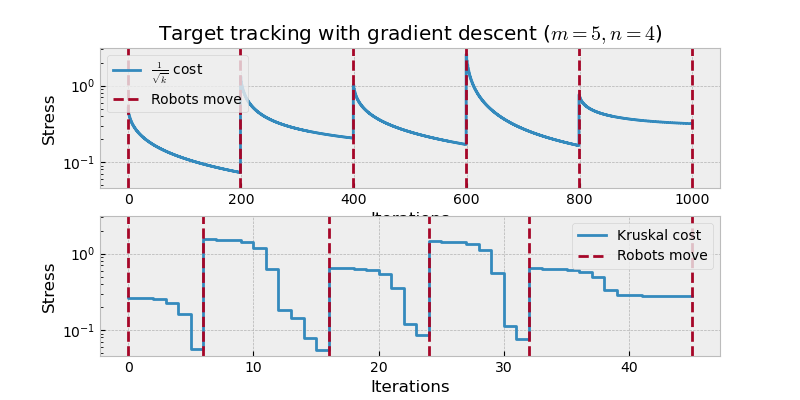
\includegraphics[width=\textwidth,trim=50 0 50 10, clip]{kruskal_5_4.png}
%         \caption{Smaller tracking example with $n=4$ robots and $m=5$ measurements}
%     \end{subfigure}
%     \begin{subfigure}{\linewidth}
%         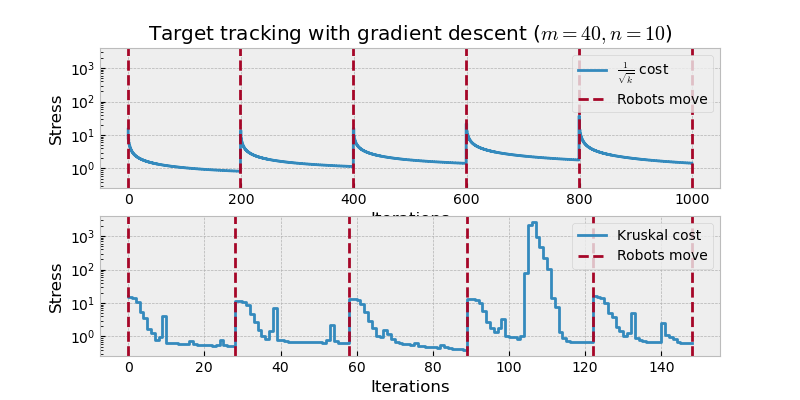
\includegraphics[width=\textwidth,trim=50 0 50 10, clip]{kruskal_40_10.png}
%         \caption{Larger tracking example with $n=10$ robots and $m=40$ measurements}
%     \end{subfigure}
%     \caption{Two different cases of robot tracking. } \label{fig:kruskal}
% \end{figure}
\begin{figure}[ht]
    \centering
    \includesvg[width=\linewidth]{kruskal.svg}
    \caption{Comparison of convergence speeds for the different algorithms.}
    \label{fig:kruskal}
\end{figure}
The plots above cover a range of reasonable values for $n$ and $m$. For values larger than this, the Riemannian elevator takes too much time and memory to run. While the difference in speed is not large, it should be noted that Kruskal's algorithm requires virtually no tuning, while the other two step schedules required tuning to achieve good performance. Nonetheless, it is not a large improvement and is not key to the success of the tracking algorithm. 

In figures~\ref{fig:point-est-small} and~\ref{fig:point-est-large}, the point estimation from distance measurements is showcased. A number of points were generated with noisy distance measurements between them. These values were passed to the Riemannian elevator which generated an initial estimate of the positions, which were further refined by Kruskal's gradient descent method.
\begin{figure}[ht]
    \centering
    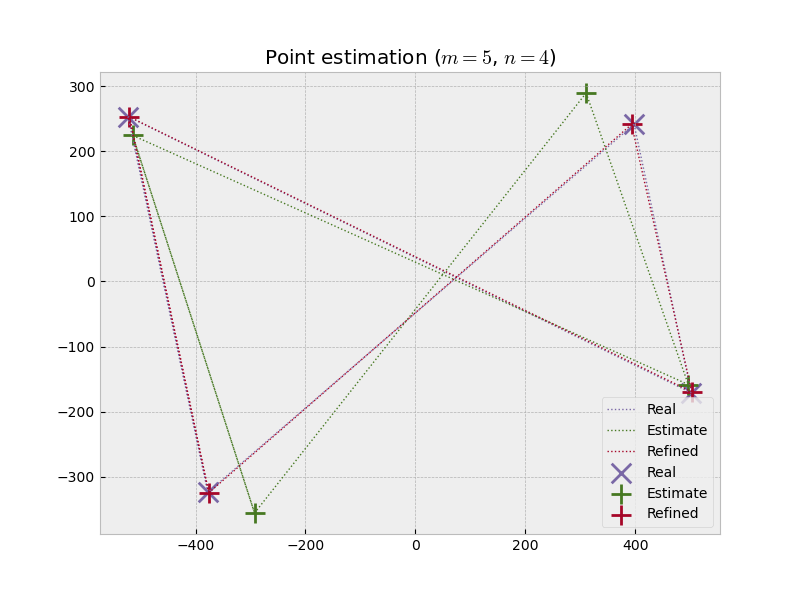
\includegraphics[width=\linewidth,trim=0 20 0 30, clip]{point_est_5_4.png}
    \caption{A smaller example of point estimation.}
    \label{fig:point-est-small}
\end{figure}
\begin{figure}[ht]
    \centering
    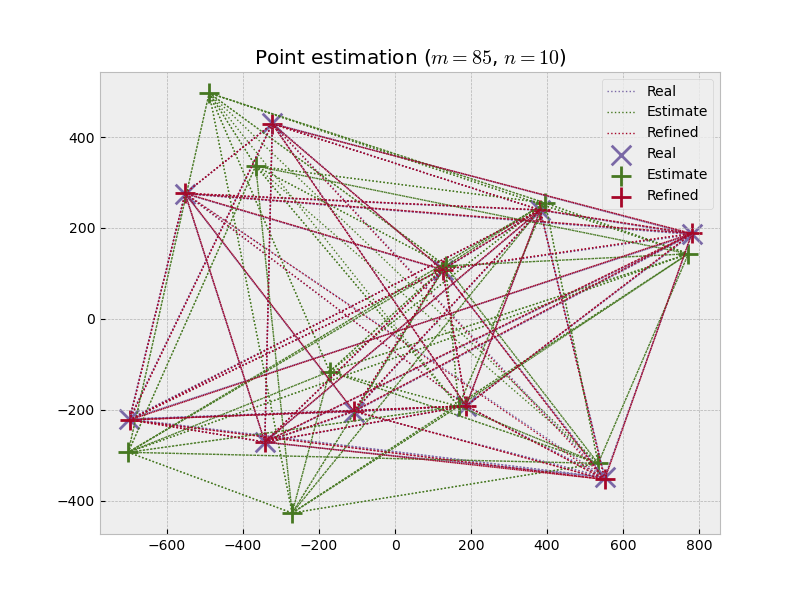
\includegraphics[width=\linewidth,trim=0 20 0 30, clip]{point_est_85_10.png}
    \caption{A larger example of point estimation.}
    \label{fig:point-est-large}
\end{figure}
% \begin{figure}[ht]
%     \centering
%     \begin{subfigure}{\linewidth}
%         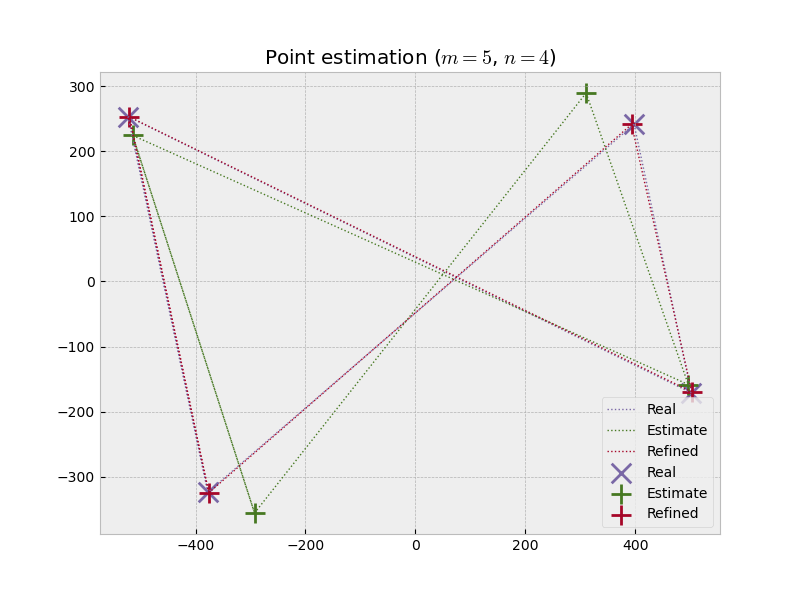
\includegraphics[width=\textwidth,trim=0 20 0 30, clip]{point_est_5_4.png}
%         \caption{A smaller example of position estimation}
%     \end{subfigure}
%     \begin{subfigure}{\linewidth}
%         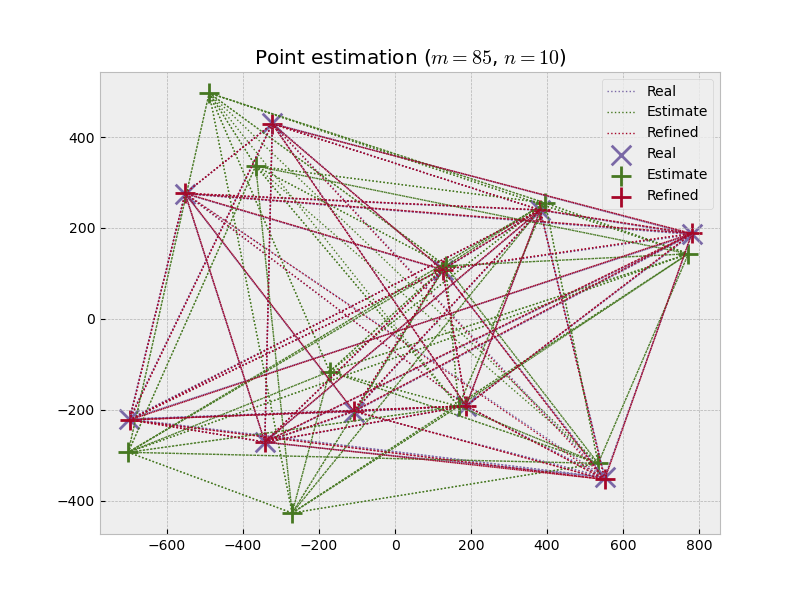
\includegraphics[width=\textwidth,trim=0 20 0 30, clip]{point_est_85_10.png}
%         \caption{A larger example of position estimation}
%     \end{subfigure}
%     \caption{Position estimation from only distance measurements. While there is ambiguity in the rotation and positions of the estimates, they have been rotated and translated to align with the true value for clarity.} \label{fig:riemann}
% \end{figure}
Further, in figure~\ref{fig:RE-accuracy}, we see the overall accuracy performance of the combined Riemannian elevator and gradient descent. For a graph with a given number of vertices $n$, the number of ways to connect two of the vertices with a directed edge is given by 
\begin{align}
    P(n, 2) = \frac{n!}{(n-2)!} = n (n-1)
\end{align}
Therefore, we can determine experimentally that at fewer vertices, $50\%$ accuracy is achieved when around $50\%$ of the possible edges are utilized. As the number of vertices grows, the number of required edges for $50\%$ accuracy shrinks down to about $30\%$. While this is in no way conclusive, and obviously dependant on the level of noise, it does show the power of the Riemannian elevator. 
\begin{figure}[ht]
    \centering
    \includesvg[width=\linewidth]{RE_accuracy.svg}
    \caption{These plots show the success rate of the Riemannian elevator to provide an initial point for which the subsequent gradient descent step converges to the correct arrangement of vertices.}
    \label{fig:RE-accuracy}
\end{figure}

Finally, below in figures~\ref{fig:multi-track} and~\ref{fig:single-track} are some plots of the complete tracking pipeline. It is clear that, while the system is capable of tracking positions with noisy incomplete measurements, the orientation tracking performance degrades and eventually diverges with larger noise. 
\begin{figure*}
    \begin{subfigure}{0.49\linewidth}
        \includesvg[width=\linewidth]{m45_n10_s0.svg}
        \caption{$n=10, m=45$. No noise.}
        \label{fig:track-partial-noiseless}
    \end{subfigure}
    \hfill
    \begin{subfigure}{0.49\linewidth}
        \includesvg[width=\linewidth]{m45_n10_s200.svg}
        \caption{$n=10, m=45$. Large noise.}
        \label{fig:track-partial-noisy}
    \end{subfigure}
    \begin{subfigure}{0.49\linewidth}
        \includesvg[width=\linewidth]{m90_n10_s0.svg}
        \caption{$n=10, m=90$. No noise.}
    \end{subfigure}
    \hfill
    \begin{subfigure}{0.49\linewidth}
        \includesvg[width=\linewidth]{m90_n10_s200.svg}
        \caption{$n=10, m=90$. Large noise.}
    \end{subfigure}
    \caption{Sample tracking performance for $n=10$ robots with varying numbers of measurements and noise. Dashed line is ground truth, red line is estimated state.}
    \label{fig:multi-track}
\end{figure*}
\FloatBarrier
\begin{figure}[ht]
    \centering
    \includesvg[width=\linewidth]{m120_n15_s300.svg}
    \caption{Tracking $n=15$ robots with $m=120$ measurements, e.g. $57\%$ connectivity, with very large noise.}
    \label{fig:single-track}
\end{figure}

\section{Discussion}

As shown in section~\ref{sec:result}, Kruskal's method for stress minimization is fast and reliable. However, for the problem sizes investigated in this project, the speed of all implemented algorithms was fast enough that it does not matter in practice. Due to the limited speed and memory of the laptop that all tests and simulations were carried out on, larger problem sizes were not feasible to run the Riemannian elevator on because of the SDP optimization step. While this is the case, it should still be noted that Kruskal's method is fast and stable for all problem sizes investigated, and seems likely to remain so should much larger problems be investigated. 

While the Riemannian is more reliable than a random initial guess, the difference is smaller than expected. When the comparatively long runtime is factored in, it is not unlikely that a better success rate in a shorter time might be achieved by running multiple trials of random guesses, especially if they are ran in parallel. Part of the performance gap might partially be explained by implementation details, as the gradient descent steps were implemented in an optimized fashion specifically for this problem, while the SDP and manifold optimization steps used the general-purpose solver libraries CVXPY~\cite{cvxpy1,cvxpy2} and Pymanopt~\cite{pymanopt}, respectively. It is likely that the computational limit on problem size would be possible to circumvent by using another solver algorithm or library. 

The algorithm developed for this project works insofar as it often manages to track the trajectories of the robots most of the time. However, as there is no guarantee that the EKF will not diverge, adding an additional step where the filter is reset and the Riemannian elevator is ran again if the stress is too large would help in assuring that the estimations stay correct. Another way to improve the tracking is to replace the EKF with another Kalman filter extension such as the unscented Kalman filter (UKF), as there is some evidence that the estimations from it are better.

\section{Disclosure}

This is a joint project in the courses "AA273: State Estimation and Filtering for Robotic Perception" and "EE364b: Convex Optimization II". While the two reports share some parts of the background, the main focus is different; tracking for one, and optimization methods for the other.

\section{Codebase}

The codebase of this entire project, including this report, can be found on GitHub at \url{https://github.com/erikvah/spring-project}. 

\printbibliography

\end{document}

